\documentclass[a4paper, fontsize=11pt]{scrartcl} % A4 paper and 11pt font 
\usepackage[a4paper,left=3cm,right=2cm,top=2.5cm,bottom=2.5cm]{geometry}

\usepackage[T1]{fontenc} % Use 8-bit encoding that has 256 glyphs
\usepackage{fourier} % Use the Adobe Utopia font for the document - comment this line to return to the LaTeX default
\usepackage[spanish]{babel} % Spanish language/hyphenation
\selectlanguage{spanish}
\usepackage[utf8]{inputenc}
\usepackage{amsmath,amsfonts,amsthm} % Math packages
\usepackage{graphicx} % The graphicx package
\usepackage{placeins}
\usepackage{caption}
\usepackage{subcaption}


\usepackage{listings} % Insert Scripts
\usepackage{color} %red, green, blue, yellow, cyan, magenta, black, white
\definecolor{mygreen}{RGB}{28,172,0} % color values Red, Green, Blue
\definecolor{mylilas}{RGB}{170,55,241}

\lstset{language=Matlab,%
	%basicstyle=\color{red},
	breaklines=true,%
	morekeywords={matlab2tikz},
	keywordstyle=\color{blue},%
	morekeywords=[2]{1}, keywordstyle=[2]{\color{black}},
	identifierstyle=\color{black},%
	stringstyle=\color{mylilas},
	commentstyle=\color{mygreen},%
	showstringspaces=false,%without this there will be a symbol in the places where there is a space
	numbers=left,%
	numberstyle={\tiny \color{black}},% size of the numbers
	numbersep=9pt, % this defines how far the numbers are from the text
	emph=[1]{for,end,break},emphstyle=[1]\color{red}, %some words to emphasise
	%emph=[2]{word1,word2}, emphstyle=[2]{style},    
}

\usepackage{sectsty} % Allows customizing section commands
%\allsectionsfont{\centering \normalfont\scshape} % Make all sections centered, the default font and small caps

\usepackage{fancyhdr} % Custom headers and footers
\pagestyle{fancyplain} % Makes all pages in the document conform to the custom headers and footers
\fancyhead{} % No page header - if you want one, create it in the same way as the footers below
\fancyfoot[L]{} % Empty left footer
\fancyfoot[C]{} % Empty center footer
\fancyfoot[R]{\thepage} % Page numbering for right footer
\renewcommand{\headrulewidth}{0pt} % Remove header underlines
\renewcommand{\footrulewidth}{0pt} % Remove footer underlines
\setlength{\headheight}{13.6pt} % Customize the height of the header

\numberwithin{equation}{section} % Number equations within sections (i.e. 1.1, 1.2, 2.1, 2.2 instead of 1, 2, 3, 4)
\numberwithin{figure}{section} % Number figures within sections (i.e. 1.1, 1.2, 2.1, 2.2 instead of 1, 2, 3, 4)
\numberwithin{table}{section} % Number tables within sections (i.e. 1.1, 1.2, 2.1, 2.2 instead of 1, 2, 3, 4)

%\setlength\parindent{0pt} % Removes all indentation from paragraphs - comment this line for an assignment with lots of text

\newenvironment{myalign}{\par\nobreak\large\noindent\align}{\endalign} %Altering fontsize in equations globally

%----------------------------------------------------------------------------------------
%	TITLE SECTION
%----------------------------------------------------------------------------------------

\newcommand{\horrule}[1]{\rule{\linewidth}{#1}} % Create horizontal rule command with 1 argument of height

\title{	
	\normalfont \normalsize 
	\textsc{Master en Automática y Robótica - UPM} \\ [25pt] % Your university, school and/or department name(s)
	\horrule{0.5pt} \\[0.4cm] % Thin top horizontal rule
	\huge Linear Quadratic Regulator \\ % The assignment title
	\horrule{2pt} \\[0.5cm] % Thick bottom horizontal rule
}

\author{Jorge Camarero Vera - 07052} % Your name

\date{\normalsize\today} % Today's date or a custom date

\begin{document}
	\maketitle
	
	\section{Explicación de la tarea}
	
	La finalidad de esta tarea es calcular el \textbf{LQR} para el sistema (\ref{TransferFunction}), añadiéndole un ruido blanco.\\
	
	\begin{myalign}
		G(s) = \dfrac{1}{(s+1)(s+2)(s+5)}
		\label{TransferFunction}
	\end{myalign}
	
	\subsection{Desarrollo de la tarea}
	
	Calculamos el modelo en el espacio de estados en forma canónica discreta de la siguiente forma:
	
	\begin{lstlisting}
	% Transfer Function Numerator
	num = [1];
	% Transfer Function Denominator
	den = poly([-1 -2 -5]);
	% Convert from transfer function to state-space model
	[A B C D] = tf2ss(num, den);
	sys = ss(A,B,C,D);
	% Convert continous-time state-space model to discrete-time state-space model.
	Ts = 0.1; sys_d = c2d(sys, Ts);
	
	sys_d
	
	sys_d =
	
	a = 
	x1        x2        x3
	x1    0.3982    -1.176   -0.6689
	x2   0.06689    0.9333  -0.03843
	x3  0.003843   0.09764    0.9986
	
	b = 
	u1
	x1    0.06689
	x2   0.003843
	x3  0.0001369
	
	c = 
	x1  x2  x3
	y1   0   0   1
	
	d = 
	u1
	y1   0
	
	Sample time: 0.1 seconds
	Discrete-time state-space model.
	\end{lstlisting}
	
	Se emplea la función \textit{tf2ss} para convertir la función de transferencia (\ref{TransferFunction}) en el espacio de estados. Y la función \textit{ss} para organizar las matrices del espacio de estados en un objeto de \textit{Matlab} para manejar más fácilmente modelos en el espacio de Estados. Para obtener el modelo discreto empleamos la función \textit{c2d} empleando un tiempo de muestreo de $T_s = 0.1$ segundos.\\
	
	Para calcular la matriz $K$ de la realimentación primero habrá que aplicar el siguiente algoritmo iterativo:
	
	\begin{myalign}
		\begin{split}
			&K(i) = [R + B^tP(i+1)B]^{-1} B^tP(i+1)A\\
			&u^*(i)=-K(i)x(i)\\
			&P(i) = Q + K^t(i)RK(i)+[A-BK(i)]^tP(i+1)[A-BK(i)]\\
			&J^*_i=x^t(i)P(i)x(i)
		\end{split}	
	\end{myalign}
	%
	comenzando la iteración con:
	
	\begin{myalign}
		\left . 
		\begin{matrix} 
			K(N)=0 \\
			P(N)=Q
		\end{matrix}
		\right \}
		\Longleftrightarrow P(N+1)=0
	\end{myalign}
	
	Para implementar este algoritmo se ha desarrollado un algoritmo para probar distintas variaciones de la matriz $Q$ para comprobar cómo varían los resultados. Pero para una primera etapa de desarrollo se ha definido $Q = Identidad$ y $R = 1$, quedando:
	
	\begin{lstlisting}
	K_ = zeros(1,3);
	K = ones(1,3);
	P = zeros(3,3);
	R = 1;
	Q = eye(3);
	while 1
		K_ = K;
		K = inv(R + sys_d.b' * P * sys_d.b) * sys_d.b' * P *...
		sys_d.a;
		P = Q + K' * R * K + (sys_d.a - sys_d.b * K)' * P *...
		(sys_d.a - sys_d.b * K);
		if abs(K - K_) < [0.001 0.001 0.001]
			break;
		end;
	end;
	
	K =
	
	0.0480    0.0342    0.0093
	\end{lstlisting}
	
	Con estos resultados de $K$ desarrollo el modelo, Figura \ref{Model}, para obtener una salida final no nula regulada.
	
	\begin{figure}[h!]
		\centering
		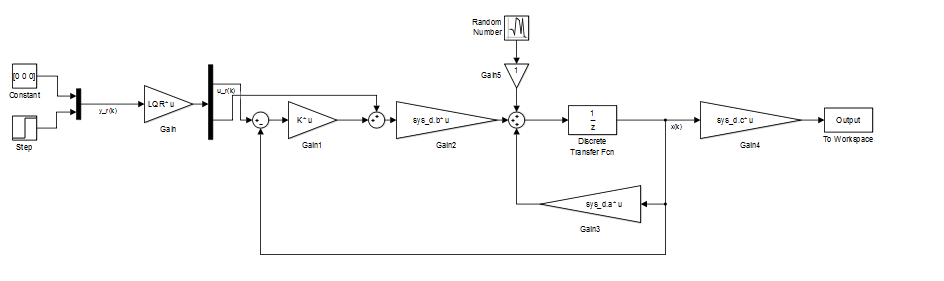
\includegraphics[width=1.0\linewidth]{images/Model.png}
		\caption{Modelo regulado mediante LQR empleado en la simulación.}
		\label{Model}
	\end{figure}
	\FloatBarrier
	%
	Como matriz LQR del modelo se emplea:
	
	\begin{lstlisting}
	LQR = inv([sys_d.a-eye(3) sys_d.b; sys_d.c 0])
	
	LQR =
	
	-0.5663    9.8593   -0.0827   -0.0000
	0.0083   -0.5002    9.9999   -0.0000
	0         0         0    1.0000
	9.9999   79.9164  174.9999   10.0000
	\end{lstlisting}
	
	Ante una entrada escalón con valor estacionario de $80$ y ruido con varianza, $\sigma^2 = 0.6$ se obtiene la respuesta de la Figura 
	
	\begin{lstlisting}
	sim('LQR_Model');
	plot(Output)
	\end{lstlisting}
	
	\begin{figure}[h!]
		\centering
		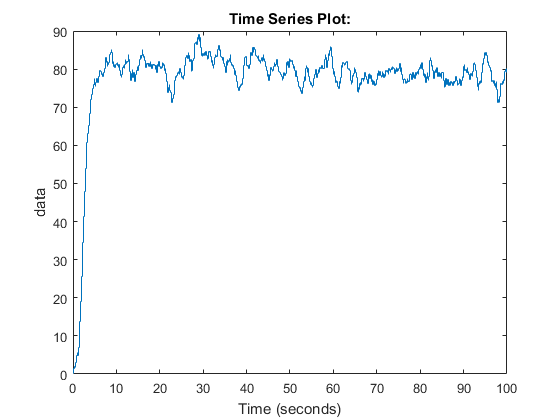
\includegraphics[width=1.0\linewidth]{images/Output.png}
		\caption{Salida regulada mediante LQR.}
		\label{Output}
	\end{figure}
	\FloatBarrier
	
	En la elaboración de esta tarea los únicos parámetros escogidos aleatoriamente han sido $Q$ y $R$, por lo que se ha elaborado este algoritmo para testear distintos valores:
	
	\begin{lstlisting}
	figure
	for i = 1:10
		K_ = zeros(1,3);
		K = ones(1,3);
		P = zeros(3,3);
		R = 5*randn + 10;
		Q = 5*randn(3,3)+10;
		while 1
			K_ = K;
			K = inv(R + sys_d.b' * P * sys_d.b) * sys_d.b' * P * sys_d.a;
			P = Q + K' * R * K + (sys_d.a - sys_d.b * K)' * P * (sys_d.a - sys_d.b * K);
			if abs(K - K_) < [0.001 0.001 0.001]
				break;
			end;
		end;
		sim('LQR_Model');
		hold on
		plot(Output)
	end;
	\end{lstlisting}
	
	\begin{figure}[h!]
		\centering
		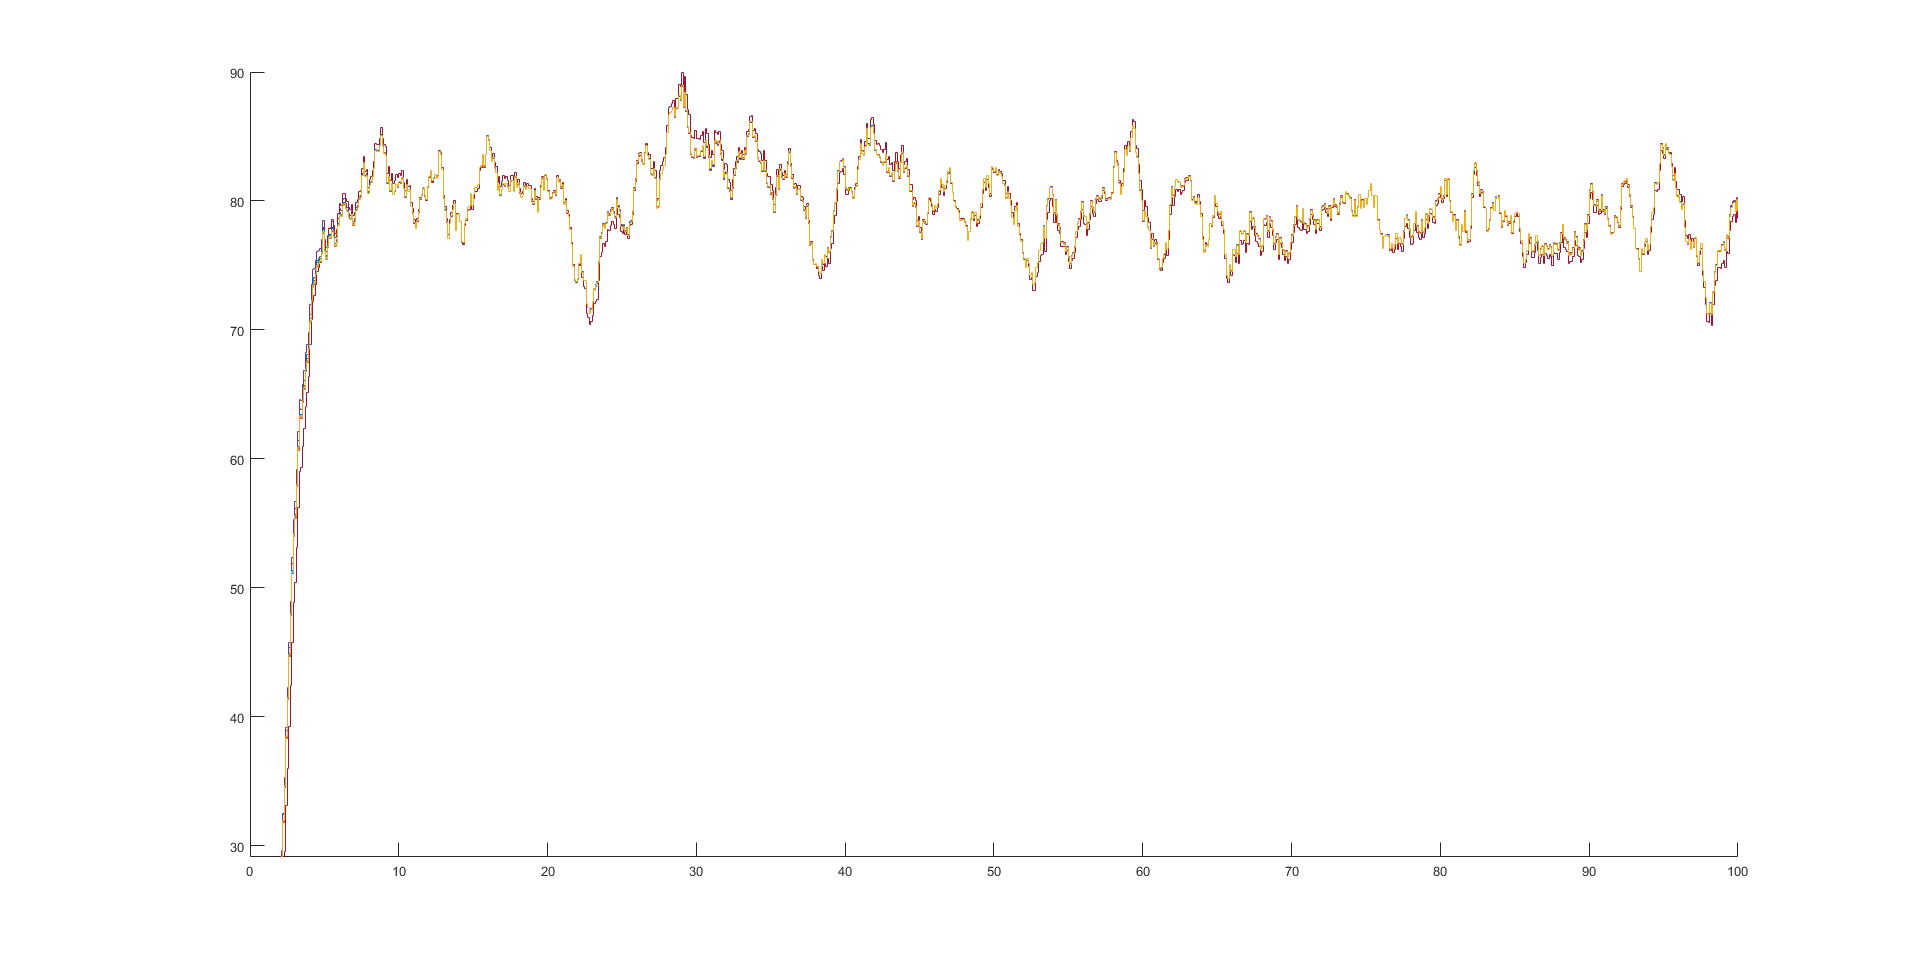
\includegraphics[width=1.0\linewidth]{images/Outputs.png}
		\caption{Salidas regulada mediante LQR ante valores aleatorios de $Q$ y $R$.}
		\label{Outpust}
	\end{figure}
	\FloatBarrier
	%
	Se observa que apenas hay variación por la elección de distintas variables $Q$ y $R$. (Si tuviera tiempo me gustaría averiguar porqué esto sucede.)
	
\end{document}